



\begin{figure*}[!bp]
    \caption{Receiver Operator Curves}\label{fig:roc}
    \centering
    \begin{subfigure}[b]{0.49\textwidth}
        \caption{In Sample}
        \centering
        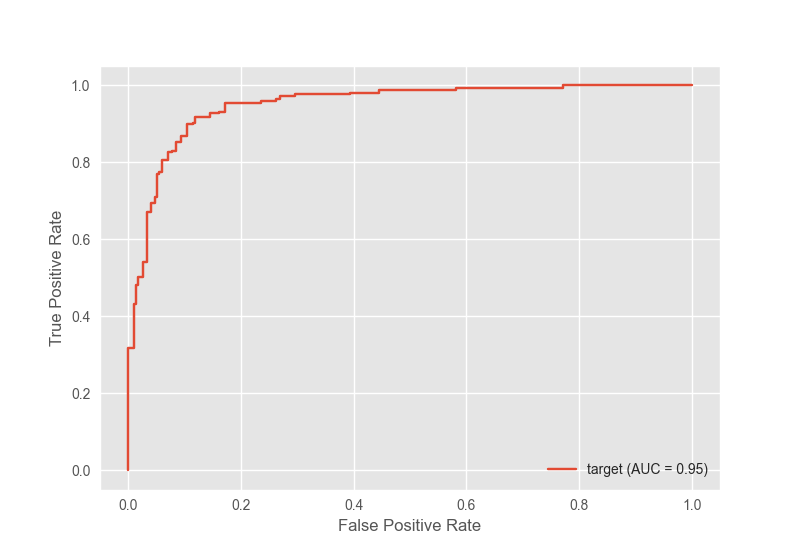
\includegraphics[width=\textwidth]{plots/roc-is-1.png}
    \end{subfigure}
    \begin{subfigure}[b]{0.49\textwidth}
        \caption{Out of Sample}
        \centering
        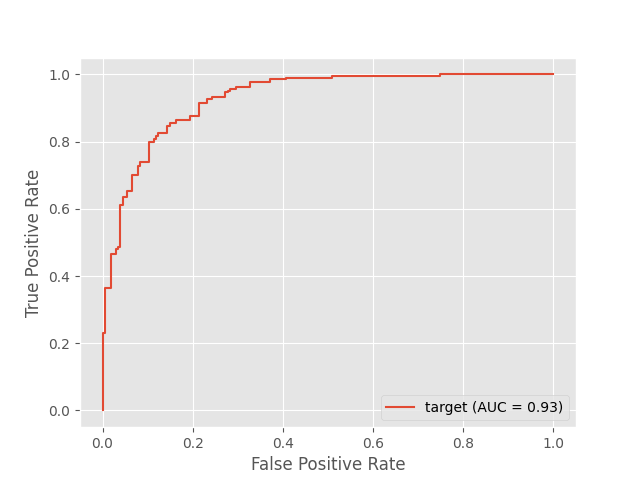
\includegraphics[width=\textwidth]{plots/roc-oos-1.png}
    \end{subfigure}
\end{figure*}

When predicting in sample, the model had a log-loss score of $0.2862$, a Brier score of $0.0836$, and an AUC of $0.9501$, indicating that the model predicts well in sample. 
After training the model, a receiver operating characteristic analysis was applied to determine the optimal threshold for predicting the target. 
To calculate the ROC metrics, a confusion matrix was created for each hundredth between $0$ and $1$. 
The selected threshold was $0.5$ with an accuracy of $0.9008$, a precision of $0.8930$, a sensitivity of $0.9182$, and a specificity of $0.8822$.
When predicting out of sample, the model had a log-loss score of $0.3406$, a Brier score of $0.1073$, and an AUC of $0.9294$, indicating that the model does not lose much generality when introduced to new data. 
Figure~\ref{fig:roc} shows the in sample and out of sample receiver operator curves.